\subsection{Justification VGA}

One challenge was the image rendering on the VGA-screen. Since a
pre-stored background image is being used, it was decided that the
easiest way to implement the signal level indicators with a gradient
was to create a background image containing filled bars and render
black over the parts that should not be filled rather than having the
application draw the bar itself.

\begin{figure}[H]
        \centering 
        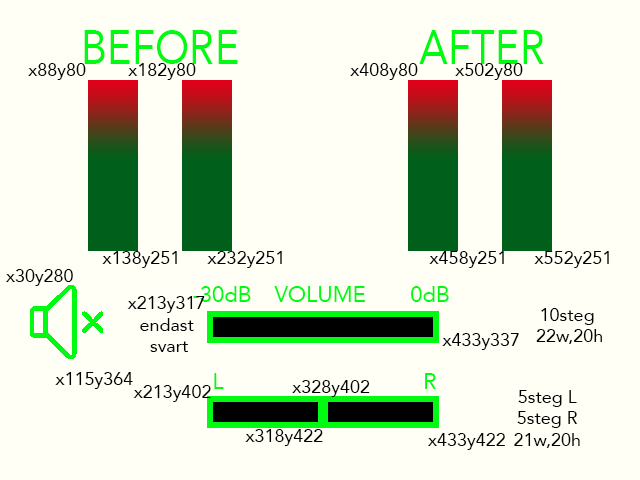
\includegraphics[scale=1.00]{fig/picture_xy.png}
        \caption{Concept UI image}
        \label{fig:picture_xy}
\end{figure}

Figure \ref{fig:picture_xy} is a concept version of the image
used. Constants were declared using the coordinates of the upper right
corner of the bars displaying signal level, both right and left
channel before manipulation, the volume bar and the mute symbol and
the width height and offset to the remaining bars. This way conditions
could be defined for when \verb+hcnt+ and \verb+vcnt+ coordinates were
inside the bars or not.

The input consists of four 8 bit unsigned with values spanning from 0
to 171 that holds information about the signal level bars, a 4 bit
unsigned for volume setting spanning from 0 to 9 and a 5 bit signed
value for balance setting spanning from -8 to 8.

For the signal level bars the application checks that \verb+hcnt+ and
\verb+vcnt+ is in the bar and then compares the \verb+vcount+ value with
(171 -- input)
(which will represent the part of the bar that should be
painted over). And if \verb+hcnt+ and \verb+vcnt+ is in the correct
area the output \verb+render_bar+ is set high and black will be rendered in
the affected pixel.

The volume bar works in a similar way but the input is multiplied with
a constant declaring the width of the boxes, and checking towards
\verb+hcnt+ instead since the bar is positioned horizontally rather
than verticaly.

The balance works as volume with the exception that it is divided in two
parts, one representing the right side being filled and one
representing the left.

There is also support for peak level indicators. They are represented
by 8 bit unsigned internal signals that are assigned the bar value iff
the current bar value is greater than the last value assigned. A
counter counting 50k clock cycles is then decremented before the peak
level amplitude is decremented. The application draws the peak level
line in the same manner as for the bars, but setting the output
\verb+render_peak+ high instead to give the peak level indicator a
different color than the one generated from \verb+render_bar+.

Since the application used in \emph{laboration 2} also rendered a background image
stored in the SRAM only minor ajustments needed to be done. The
sub module \verb+bar_tender+ described above sets \verb+render_bar+ and
\verb+render_peak+ high in the affected pixels and the submodule
\verb+bar_mixer+ works as a multiplexer forwarding color-information
from SRAM when \verb+render_bar+ and \verb+render_peak+ are set
low. And forwards black (for bars) and white (for peak) when the
inputs are set high.

The mute symbol is implemented simply by drawing a black square over
the symbol whenever the \verb+mute+ input is set low.
 
